
\section{JSBMLInterface package}

In questa sezione descriveremo il package \textbf{JSBMLInterface}.

Questo package contiene le implementazioni dei concetti che riguardano
l'interfacciamento con il modello SBML e in particolare con la
libreria JSBML \footnote{aggiungere riferimento bibliografico al link
  della libreria}. 

\subsection{Supplied Abstractions}

Le astrazioni fornite da questo package sono le seguenti:
\begin{itemize}
\item astrarre dalla libreria JSBML e dal suo modello dati. In questo
  modo l'unico contesto del progetto dipendente dalla libreria JSBML
  \`e confinato a questo singolo package. Questo permette agli altri
  package di non essere a conoscenza della specifica "sorgente" che
  fornisce il modello, in quanto se si vorr\`a sostituire libreria di
  interfacciamento con modelli SBML, sar\`a necessario apportare le
  modifiche solo in questo package, lasciando tutto il restante codice
  del progetto inalterato.
\item interpretare il modello fornito dalla libreria JSBML, costruire
  gli elementi fondamentali del nostro modello dati e renderlo
  disponibile per iniziare successive computazioni.
\end{itemize}

\subsection{Class diagram}

Riporto una versione semplificata del diagramma delle classi di questo
pacchetto, disegnando solo quelle classi di interesse per la
trattazione.
\begin{figure}
  \centering
  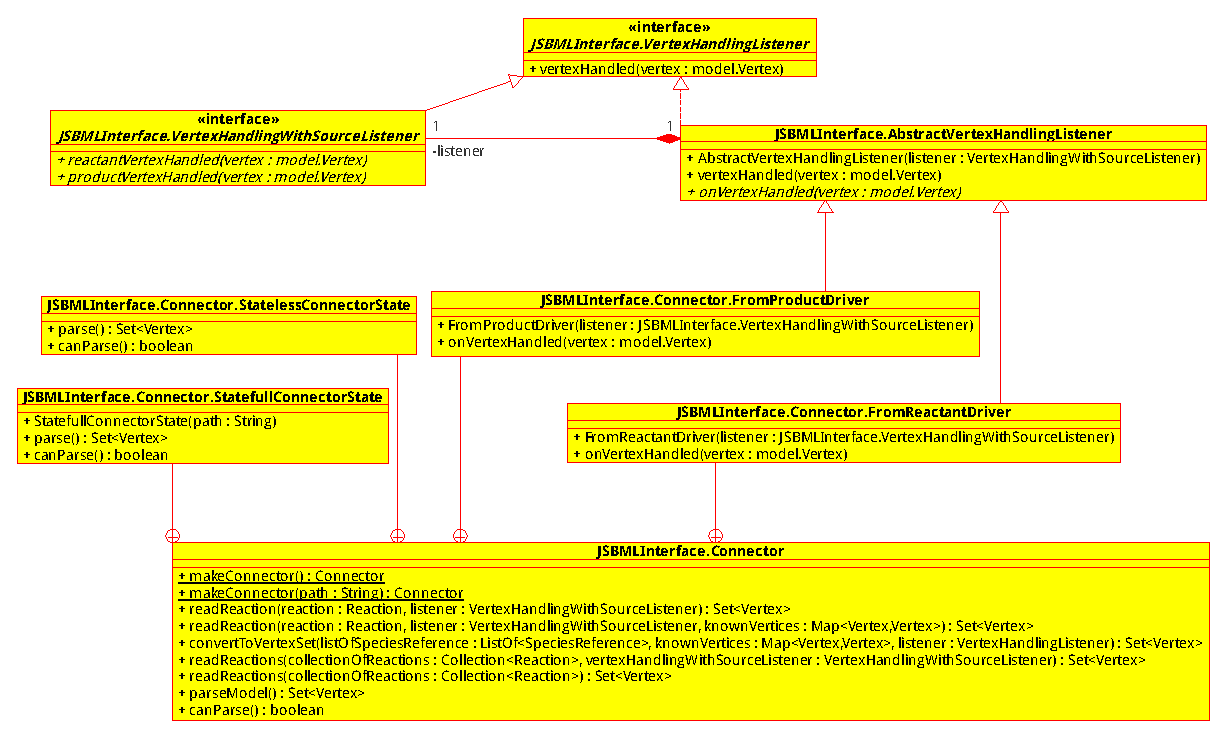
\includegraphics[angle=90]{packages/JSBMLInterface-class-diagram.eps}
  \caption{JBSMLInterface package's classes}
  \label{fig:JSBMLInterface-ClassDiagram}
\end{figure}

In questo package la classe principale e che merita qualche
spiegazione \`e \emph{Connector}.

Questa classe incapsula la responsabilit\`a di delegare alla libreria
JSBML la lettura di un modello SBML e successivamente interpretare il
risultato di tale lettura in modo da costruire un nostro modello dati
interno, input di successive computazioni.

La parte di interpretazione del modello letto dalla libreria JSBML \`e
quella pi\`u interessante, in quanto permette di elaborare e
selezionare solo quelle informazioni del modello SBML che
effettivamente sono necessarie al nostro lavoro, come descritto nella
sezione "\nameref{sec:necessaryRealObjectsModeledInSBML}". 

Questo procedimento \`e implementato principalmente nel metodo
\emph{readReactions}, il quale permette di costruire un insieme di
vertici che verranno usati per costruire il nostro modello di dominio,
a partire da una collezione di reazioni, risultato della lettura della
libreria SBML. Inoltre, come spiegher\`o nella prossima sezione, \`e
possibile passare come argomento un \emph{listener} da notificare ogni
qualvolta si costruisce un nuovo vertice per il modello da costruire.

Quello che viene fatto \`e di scandire ogni reazione e, per ognuna, si
creano tanti vertici tanti sono gli oggetti appartenenti agli insiemi
\emph{reactants} e \emph{products}, prestando attenzione a non
costruire nuovi vertici per species gi\`a analizzate.

\section{Patterns and coding idioms}

\subsection*{Description}
In questa sezione scrivo una breve descrizione di un interessante
\emph{coding idiom} che ho implementato.
\begin{description}
\item[Problem] Si invoca un metodo il quale ha un parametro con un
  determinato tipo. Questo parametro permette di modellare due
  concetti diversi con lo stesso oggetto. Quello che si vuole \`e di
  poter abilitare un client di ascoltare la computazione ed essere
  notificato usando un oggetto listener sul metodo relativo alla
  specializzazione del concetto che si sta usando attualmente.
\item[Forces] Si vogliono rispettare questi requisiti:
  \begin{itemize}
  \item mantenere una firma del metodo con il parametro di tipo che
    astrae dai diversi concetti. In questo modo il codice non dipende
    dal concetto specifico ma rimane generico.
  \item il client vorrebbe essere notificato non in maniera generica,
    ma sapere quando viene usato un concetto e quando ne viene usato
    uno diverso. L'interfaccia su cui vorrebbe essere notificato il
    listener viene fornita dal client e la possiamo vedere come un
    contratto. 
  \item nel contesto nel quale avviene l'innesco della computazione
    \`e possibile stabilire la natura dei concetti che verranno
    manipolati.
  \end{itemize}
\item[Solution] Per risolvere il problema introduciamo una classe
  astratta che implementa il generico metodo di handling e che
  incapsula il listener fornito dal client, agendo come un
  \emph{wrapper}. Il metodo che esegue la computazione, quando
  incontra un oggetto che modella un concetto, di cui non siamo a
  conoscenza del tipo a \emph{compile time}, invia un messaggio al
  listener. Ma non sar\`a il listener fornito dal client a rispondere
  a tale messaggio, bensi il wrapper. Ma, essendo il wrapper una
  classe astratta, l'oggetto che effettivamente risponder\`a potr\`a
  notificare il vero listener, invocando un messaggio che cattura lo
  specifico concetto che \`e stato elaborato. Lo specifico
  implementatore della classe astratta viene costruito e passato come
  argomento nel contesto in cui \`e possibile sapere il tipo di
  concetti che verranno elaborati dal metodo generico.
\end{description}

\subsection*{Reification}
Nella mia implementazione il metodo generico che esegue la
computazione \`e \emph{convertToVertexSet}, il quale ha come parametro
che astrae su due concetti diversi, \emph{listOfSpeciesReference}. 

La computazione eseguita dal metodo \`e di creare un nuovo vertice
ogni qualvolta si trova una species non ancora analizzata, e di
notificare questo vertice al client, tramite il listener passato come
argomento.

\begin{lstlisting}
  public Set<Vertex> convertToVertexSet( 
  ListOf<SpeciesReference> listOfSpeciesReference, 
  Map<Vertex, Vertex> knownVertices,
  VertexHandlingListener listener) 
\end{lstlisting}
Come si vede la firma di questo metodo \`e molto generica, in quanto
il parametro \emph{listOfSpeciesReference} una volta pu\`o contenere
una lista di \emph{reactants}, altre volte una lista di
\emph{products}. Inoltre il listener che viene usato, non mette a
disposizione metodi che catturano il tipo di un concetto specifico,
bensi permette solo di notificare che \`e stato elaborato un vertice,
ma non possiamo sapere se questo \`e un \emph{reactants} o un
\emph{products}.

\`E quindi possibile implementare l'idea data nella parte "Solution",
instanziando il corretto specializzatore della classe astratta nel
contesto dove \`e possibile sapere se si sta per analizzare una
collezione di \emph{reactants} oppure di \emph{products}: questo \`e
possibile farlo nel metodo \emph{readReaction}. Riporto sotto il
momento della creazione del corretto wrapper:
\begin{lstlisting}
Set<Vertex> reactants = this.convertToVertexSet(
				reaction.getListOfReactants(), knownVertices,
				new FromReactantDriver(listener));

Set<Vertex> products = this.convertToVertexSet(
				reaction.getListOfProducts(), knownVertices,
				new FromProductDriver(listener));
                              \end{lstlisting}
Quello che i due wrapper eseguiranno quando verr\`a invocato il metodo
astratto della classe astratta, sar\`a quello di notificare sul
relativo metodo del listener il vertice ricevuto dalla classe
astratta:
\begin{lstlisting}
public abstract class AbstractVertexHandlingListener implements
		VertexHandlingListener {

	private final VertexHandlingWithSourceListener listener;

	protected VertexHandlingWithSourceListener getListener() {
		return listener;
	}

	@Override
	public void vertexHandled(Vertex vertex) {
		this.getListener().vertexHandled(vertex);
		this.onVertexHandled(vertex);
	}

	public abstract void onVertexHandled(Vertex vertex);
}

  protected class FromReactantDriver extends AbstractVertexHandlingListener {

		@Override
		public void onVertexHandled(Vertex vertex) {
			this.getListener().reactantVertexHandled(vertex);
		}
	}

protected class FromProductDriver extends AbstractVertexHandlingListener {

		@Override
		public void onVertexHandled(Vertex vertex) {
			this.getListener().productVertexHandled(vertex);
		}
	}
\end{lstlisting}